%  !TeX  root  =  user_guide.tex 

\section{Dxf2Shp Converter Plugin}

% when the revision of a section has been finalized, 
% comment out the following line:
%\updatedisclaimer

The dxf2shape converter plugin can be used to convert vector data from DXF to Shapefile 
format. It requires the following parameters to be specified before running:

\begin{itemize}
\item \textbf{Input DXF file}: Enter path to the DXF file to be converted
\item \textbf{Output Shp file}: Enter desired name of the Shapefile to be created
\item \textbf{Output file type}: Specify the geometry type of the output Shapefile. 
Currently supported types are polyline, polygon, and point.
\item \textbf{Export text labels}: When this checkbox is enabled, an additional Shapefile point layer will be created, and the associated dbf table will contain information about the "TEXT" fields found in the dxf file, and the text strings themselves.
\end{itemize}

\begin{figure}[ht]
   \centering
   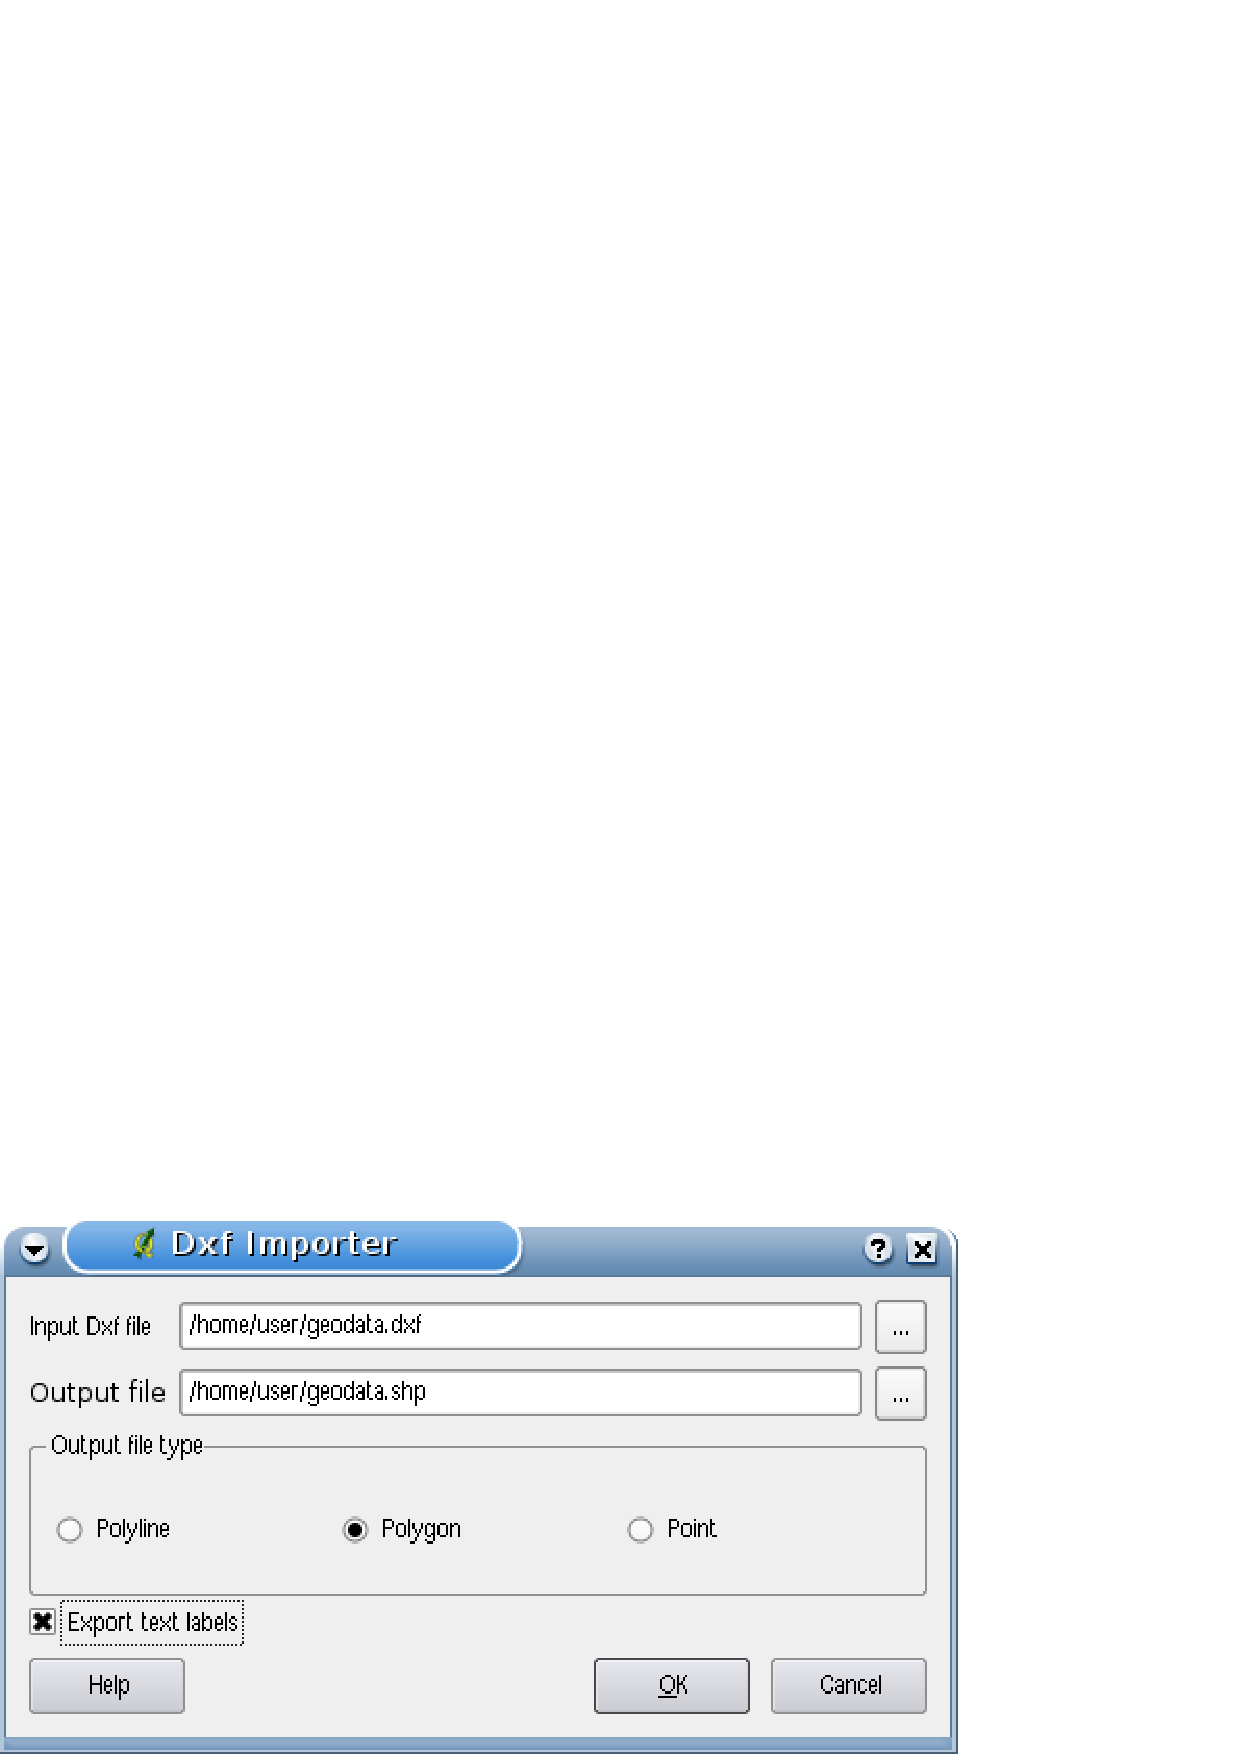
\includegraphics[clip=true, width=12cm]{dxf2shape_dialog}   
   \caption{Dxf2Shape Converter Plugin \nixcaption}\label{fig:dxf2shape_dialog}
\end{figure}

\minisec{Using the Plugin}

\begin{enumerate}
  \item Start QGIS, load the Dxf2Shape plugin in the Plugin Manager (see Section 
  \ref{sec:load_core_plugin}) and click on the \toolbtntwo{dxf2shp_converter}{Dxf2Shape Converter} 
  icon which appears in the QGIS toolbar menu. The Dxf2Shape plugin dialog appears as shown in Figure \ref{fig:dxf2shape_dialog}.
  \item Enter input DXF file, a name for the output Shapefile and the Shapefile type.
  \item Enable the \checkbox{Export text labels} checkbox if you want to create an extra point layer with labels.
  \item Click \button{Ok}. 
\end{enumerate}

\FloatBarrier
